\section{Derivable functions}
In this section, we state the main result of this paper, which describes  the  first-order tree-to-tree functions in terms of  certain atomic functions by using certain combinators.  A typical combinator is composition of functions.

\paragraph*{The category of ranked sets.} Even if our goal is to generate first-order tree-to-tree transductions, our basic functions will not necessarily be function transforming trees into trees. For example, we will need to manipulate pairs of trees or trees of trees etc. Clearly, these data structures are encodable by trees, however this would make the basic functions rather complex. We make the choice of introducing new types for our basic functions in order to get simple basic functions.

Among the types that we introduce, the most important one is certainly the type of \emph{terms}. This type appears when we want to decompose our trees into smaller parts, as illustrated by the figure below. Each small part of the tree is not really a tree\footnote{This is a difference of trees as opposed to strings~\cite{bojanczykRegularFirstOrderList2018}, where ranked sets are not needed, because a part of a string is also a string.}: it has dangling ports which  allows to connect it with the other parts. We call \emph{terms} such tree with ports. 
\mypic{15}
A term can naturally be seen as a ranked element, its arity being the number of its ports. Because the set of terms is itself a ranked set,  we can create terms of terms.  A consequence of using terms is that we will work in the category of ranked sets; i.e.~the types we use will be ranked sets and the functions we consider are arity-preserving functions between ranked sets. As in Section~\ref{sec:trees-transductions}, we write ranked sets in red. We also use red for operations that output ranked sets. 


 
%
%
%The crucial property of the atomic functions and  the combinators is that they use ranked sets. This is because the type constructor of this paper, namely terms, uses ranked sets.  Roughly speaking, a term is a tree with missing parts. The missing parts arise when we  isolate smaller parts of a bigger tree, as illustrated in the following picture:




%\begin{definition}[Terms]\label{def:terms}
%    An  term\footnote{
%        Our definition of terms differs from the definition used in universal algebra. An $n$-ary term in the sense of this paper is, in the language of universal algebra, a term over variables $\set{x_1,\ldots,x_n}$ where each variable appears exactly once, and the variables are used from left to right.  The requirement that variables appear  once is related to the linear output size of first-order tree-to-tree transductions. Without this requirement, even homomorphisms would have exponential output size. 
%    } over a ranked set $\rSigma$ is a tree over alphabet $\rSigma \redplus \redzero$, where $\redzero$ is a set with one element of arity zero.  The nodes with labels from $\redzero$  -- which are leaves --  are called \emph{ports}. The arity of a term is the number of ports.  We write $\tmonad \rSigma$ for the ranked set of terms over $\rSigma$.  
%\end{definition}





\paragraph*{Types.} The following definition describes the  ranked sets that will be allowed as domains and co-domains of our functions.  We call such ranked sets \emph{types}.
%  The general idea is that we start with finite ranked sets, and close these under the following type constructors: coproducts, two kinds of product (Cartesian and tensor), taking terms, and a type constructor that allows to merge ports.
%  and the matrix power. 
% The  matrix power -- which is possibly the least natural type constructor -- will be motivated and discussed in more detail later on.



\begin{definition}[Types] \label{def:types} Every  ranked set with finitely many elements is a type. The set $\ranked{\bot}$ which contains a single  element for each arity is also a type. We denote by $n$ the $n$-ary element of $\ranked{\bot}$.  Furthermore, types are closed under applying the following type constructors:
    \begin{enumerate}
    \item \emph{Terms.} An element of $\tmonad \rSigma$, the set of terms over $\rSigma$, is a tree over alphabet $\rSigma \redplus \redzero$.  The nodes with labels from $\redzero$  -- which are leaves --  are called \emph{ports}. The arity of a term is the number of ports. We draw terms like this:
            \mypic{51}
      \item \emph{Coproduct.} An element of the \emph{coproduct} $\ranked{\Sigma_1 + \Sigma_2}$ is a co-pair of the form  $(i,a)$ where $i \in \set{1,2}$ and $a \in \ranked{\Sigma_i}$. The arity is inherited from $a$. 
      
%We draw co-pairs like this:
%       \mypic{61}
              \item       \emph{Product.} An element of the   \emph{product}%\footnote{
%                  A more precise name would be \emph{tensor product}. The alternative product, call it \emph{Cartesian product}, would have as $n$-ary elements  pairs $(a_1,a_2)$ such that both $a_1$ and $a_2$ have arity $n$. Since we do not use Cartesian product, we write product without specifying that we mean the tensor product.
%              } 
 $\ranked{\Sigma_1 \otimes \Sigma_2}$  is a  pair $\tensorpair{a_1,a_2}$ where $a_i \in \ranked{\Sigma_i}$. The arity  of this pair is the sum of arities of its components $a_1$ and $a_2$. We draw pairs like this:
        \mypic{52}
        \item \emph{Folding.} For every $k \in \set{1,2,3,\ldots}$, we have a unary type constructor $\reduce k \rSigma$  which is used to reduce arities, by grouping ports into groups of size at most $k$.  An $n$-ary element of $\reduce k \rSigma$, which is called a \emph{$k$-fold}, consists of an element      $a \in \rSigma$  together with an  injective  function
            \begin{align*}
                f : \set{1,\ldots,\arity a} \to \set{1,\ldots,k} \times  \set{1,\ldots,n}.
            \end{align*}
            We denote such an element as $a/f$ and draw it like this: \mypic{53}
            If $i\in  \set{1,\ldots,\arity a}$, then the second component of $f(i)$ specifies to which group the $i$-th port of $a$ will participate, while the first component specifies its place in this group. In the picture above, the arity of $a$ is $6$, the arity of $a/f$ is $4$, and $k$, the size of the groups,  is $2$. For instance we have that $f(1)=(1,2)$, because the first port of $a$ participated to the group forming the first port of $a/f$, and because it is the second element in this group.
        \item \emph{Shallow terms.} The  ranked set $\shallowterm \rGamma \rSigma$ of  \emph{shallow terms} is defined as
        \begin{align*}
            \ranked {\shallowterm \rSigma \rGamma \eqdef \coprod_{a \in \rSigma} \underbrace{\rGamma\otimes\ldots\otimes\rGamma}_{\text{arity of $a$}}}.
        \end{align*}
        The coproduct in the above definition is infinite when $\rSigma$ is infinite. 
        An equivalent definition is that a shallow term  is the special case of  a term over $\rSigma \redplus \rGamma$ where  the root has label from $\rSigma$,  children have labels  from $\rGamma$, and grand-children are ports. We draw shallow terms like terms:
        \mypic{76}
    \end{enumerate}
\end{definition}


\newcommand{\funcitem}[3]{\ranked{#1  } &:& \ranked{#2} \rto  \ranked{#3}}
All of the type constructors  above are functors, in the sense  that  arity preserving functions
\begin{align*}
\ranked{f_1 : \Sigma_1 \to \Gamma_1 \qquad f_2 : \Sigma_2 \to \Gamma_2}
\end{align*}       
can be lifted along the type constructors to new arity preserving  functions
\begin{eqnarray}
\label{eq:liftplus}\funcitem{f_1 + f_2}{\Sigma_1 + \Sigma_2}{\Gamma_1 + \Gamma_2} \\
\funcitem{(f_1,f_2)}{\Sigma_1 \otimes \Sigma_2}{\Gamma_1 \otimes \Gamma_2}\\
\funcitem{\reduce k f_1}{\reduce k \Sigma_1}{\reduce k \Gamma_1}\\
\funcitem{\tmonad f_1}{\tmonad \Sigma_1}{\tmonad \Gamma_1}\\
\label{eq:liftshallow}\funcitem{\shallowterm{f_1}{f_2}}{\shallowterm{\Sigma_1}{\Sigma_2}}{\shallowterm {\Gamma_1}{\Gamma_2}} 
\end{eqnarray}

We now introduce the main new definition of this paper.

\begin{definition}[Derivable function]
    The class of \emph{derivable} functions is the least class which:
    \begin{itemize}
    \item contains, for every $\rSigma$, the (unique) arity preserving function $\ranked{\Sigma \to \bot}$, and all arity-preserving functions with finite domain;
        \item contains the atomic functions in Figure~\ref{fig:fo-term};
        \item is closed under  function composition and type liftings.
    \end{itemize}
\end{definition}

%
\newcommand{\fotitem}[2]{$\displaystyle #1$ & #2 \\ \\ }
\begin{figure}[h]
    \centering 
    \begin{tabular}{ll}
        \fotitem{
            \frac
            { \ranked{f : \Sigma \to \Delta} \quad \ranked{g : \Delta \to \Gamma}}
            {\ranked{g \circ f :  \Sigma \to  \Gamma}}
            }
            {
                Composition of functions.
            }
        \fotitem{
            \ranked{f : \Sigma \to \Gamma}
            }
            {
                Every arity preserving function with finite domain $\rSigma$.
            }
            \fotitem{
                \ranked{\iota_i : \Sigma_i \to \Sigma_1 + \Sigma_2}
                }
                {
                    Coprojection for $i \in \set{1,2}$.
                }
        \fotitem{
            \frac
            { \ranked{f_1 : \Sigma_1 \to \Gamma} \quad \ranked{f_2 : \Sigma_2 \to \Gamma}}
            {\ranked{f_1 \text{or} f_2 :  (\Sigma_1 + \Sigma_2) \to  \Gamma}}
            }
            {
                Co-pairing of functions.
            }
            \fotitem{
                \ranked{\pi_i : \Sigma_1 \times \Sigma_2 \to \Sigma_i}
                }
                {
                    Projection for $i \in \set{1,2}$.
                }
        \fotitem{
            \frac
            { \ranked{f_1 : \Sigma \to \Gamma_1} \quad \ranked{f_2 : \Sigma \to \Gamma_2}}
            {\ranked{(f_1,f_2) :  \Sigma \to  \Gamma_1 \times \Gamma_2}}
            }
            {
                Pairing of functions.
            }
            \fotitem{
                \ranked{\distrcart : (\Sigma_1 + \Sigma_2)\times \Gamma \to (\Sigma_1 \times \Gamma) + (\Sigma_2 \times \Gamma)}
                }
                {
                    Cartesian product distributes across coproduct.
                }
            \fotitem{
            \frac
            { \ranked{f_1 : \Sigma_1 \to \Gamma_1} \quad \ranked{f_2 : \Sigma_2 \to \Gamma_2}}
            {\ranked{ \tensorpair{f_1,f_2}  :  \Sigma_1 \otimes \Sigma_2 \to  \Gamma_1 \otimes \Gamma_2}}
            }
            {
                Lifting functions to tensors.
            }
            \fotitem{
                \ranked{\distrtensor : (\Sigma_1 + \Sigma_2)\otimes \Gamma \to (\Sigma_1 \otimes \Gamma) + (\Sigma_2 \otimes \Gamma)}
                }
                {
                    Tensor product distributes across coproduct.
                }
            \fotitem{
            \frac{ \ranked{f : \Sigma \to \Gamma}}{\ranked{\tmonad f : \tmonad \Sigma \to \tmonad \Gamma}}
            }
            {
                Lift a function from the alphabet  to terms.
            }
            \fotitem{
            \ranked{\unit_\Sigma : \Sigma \to \tmonad \Sigma}
            }
            {
                View a letter as a term.
            }
            \fotitem{
                \ranked{\flatt_\Sigma : \tmonad \tmonad \Sigma \to \tmonad \Sigma}
                }
                {
                    Flatten a term of terms into a term.
                }
                \fotitem{
                \ranked{ \composeterm :  
                \set * + \coprod_{a \in \Sigma} \overbrace{\tmonad \rSigma \otimes \cdots \otimes \tmonad \rSigma}^{\text{arity of $a$ times}} \to \tmonad \rSigma }
                }
                {
                        Compose a term from its list of children, for finite $\rSigma$.
                }
            \fotitem{
                \ranked{ \decomposeterm : \tmonad \rSigma \to 
                \set * + \coprod_{a \in \Sigma} \overbrace{\tmonad \rSigma \otimes \cdots \otimes \tmonad \rSigma}^{\text{arity of $a$ times}}}
                }
                {
                        The inverse of $\composeterm$, for finite $\rSigma$.
                }    
    
            \fotitem{
                \ancfact, \decfact  : \ranked{\tmonad(\Sigma_1+\Sigma_2) \to \tmonad(\tmonad \Sigma_1 + \tmonad \Sigma_2)}
            }
                    {
                        Ancestor and descendant factorisations.
                    }
            \fotitem{
                \ranked{\preorder : \tmonad \Sigma \to \tmonad (\rSigma + \set{\grayball, \grayballbin})}
                }
                {
                    Pre-order traversal.
                }    
            % \fotitem{
            %     \ranked{\unfold : \tmonad (\Sigma^{[k]}) \to (\tmonad \Sigma)^{[k]}}
            % }
            %     {
            %             Matrix power distributes across terms.
            %     }
    \end{tabular} 
    
    \caption{First-order term functions}
    \label{fig:fo-term}
\end{figure}

The atomic functions describe the monad structure of terms, the (graded) monad structure of folds, some obvious distributivity, commutativity and (co)projection operations. These operations are obvious in the sens that they can be guessed from  types\footnote{The (co)projection functions are canonical in a very precise way: they are the unique functions satisfying some natural digrams. We wonder if our obvious functions are also canonical in such a precise way. We leave this question for future works.}. Our list of functions contains also three less obvious operations whose definitions are  deferred to Section~\ref{sec:atomic-and-combinators}. Before giving these definitions, we state the main result of the paper. 

% \begin{example}
%     To get a feeling for the atomic functions and combinators, we derive the function
%     \begin{align*}
%     \tensorpair{a,b} \in \ranked{\rSigma^2} \qquad \mapsto \qquad  \tensorpair{b,a} \in \ranked{\rSigma^2}
%     \end{align*}
%     which witnesses commutativity of the product for pairs of the same type. The idea is to embed pairs into terms, and use simple manipulations on terms. 
%     We  draw the unique elements of the sets $\redzero$, $\redone$ and $\redtwo$ as follows:
%     \mypic{79}
%     We begin by deriving a function which maps a tensor pair into a shallow term whose root is the unique element of $\redtwo$.  This is achieved by composing the derivable functions of types 
%     \begin{align*}
%     \ranked{
%         \xymatrix{
%             \rSigma \otimes \rSigma \ar[r] &
%             (\shallowterm \redone \rSigma) \otimes (\shallowterm \redone \rSigma) \ar[r] &
%             \shallowterm{(\redone \otimes \redone)}  {(\rSigma+\rSigma)} \ar[r] & \shallowterm \redtwo \rSigma
%         }
%     }
%     \end{align*}
%     which is described in the following picture:
%     \mypic{78}
%     The last function applies the bijection $\ranked{\redone \otimes \redone \to \redtwo}$, which is derivable by virtue of having a finite domain. 

%     Next, we can swap the children of 
% \end{example}

% We first observe that terms and unary folding are monads. 
% The monad structure for terms is induced by:
% \begin{align*}
%         \underbrace{\ranked {\tmonad f : \tmonad \Sigma \to \tmonad \Gamma}}_{\text{$\tmonad$ is a functor}} \qquad  \underbrace{\unit_\rSigma : \rSigma \rto \tmonad \rSigma}_{\text{the unit in the monad}} \qquad  \underbrace{\flatt_\rSigma : \tmonad \tmonad \rSigma \rto \tmonad \rSigma}_{\text{the product operation in the monad}},
% \end{align*}
% and a similar situation holds for unary folds $\reduce 1$.  More generally, the family of folds $\set{\reduce k}_{k}$ is a graded monad. Finally, the operation $\tmonad \reduce 1 \rSigma \rto \reduce 1 \tmonad \rSigma$ is a distributive law of these two monads.

% For a derivable function, its domain and co-domain are types as in Definition~\ref{def:types}, in particular the domain and co-domain are ranked sets. The atomic functions are arity-preserving and the combinators preserve this property, and therefore all derivable functions are arity-preserving. 


% We are now ready to state the main theorem of this paper. 

\begin{theorem}\label{thm:main}
    Let $\rSigma,\rGamma$ be finite ranked sets. A function 
    \begin{align*}
        f : \trees \rSigma \to \trees \rGamma
    \end{align*}
    is a first-order tree-to-tree transduction if and only if it is the restriction to trees of some derivable
    \begin{align*}
        \ranked {f : \tmonad \Sigma \to \tmonad \Gamma}.
    \end{align*}
    
\end{theorem}

%\subsection{Proposition of another presentation of atomic functions}
\begin{figure}
\fbox{
\begin{minipage}{1\linewidth}
\begin{itemize}
\item \textbf{Unit.}
$$
\begin{array}{c}
 \ranked{\Sigma} \ \ \ranked{\leftrightarrow} \ \    \ranked{ \Sigma \cdot 1}\\[5pt]
        {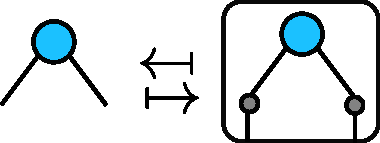
\includegraphics[scale=.4]{pictures/sigma-dot-1}} 
\end{array}
$$
\item \textbf{Associativity.}
$$
\begin{array}{c}
 \ranked{(\Sigma \cdot \Gamma)\cdot \Delta } \ \ \ranked{\to} \ \    \ranked{ \Sigma \cdot (\Gamma \cdot \Delta)}\\[5pt]
        {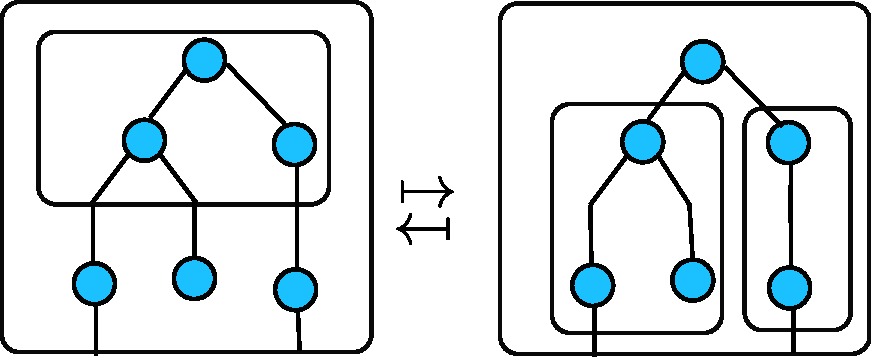
\includegraphics[scale=.4]{pictures/associativity-shallow}} 
\end{array}
$$
\item \textbf{Terms as shallow terms.}
$$
\begin{array}{c}
 \ranked {1 + \shallowterm \Sigma {\tmonad \Sigma}\ \ \to \ \  \tmonad \Sigma}\\[5pt]
        {
        \begin{tabular}{l}
            Every term is either just a port,\\ or has a root and child subterms.    
        \end{tabular}    
        }
\end{array}
$$
\item \textbf{Tensors as shallow terms.}
$$
\begin{array}{c}
\ranked {\Sigma^n \ \ \leftrightarrow \ \ \shallowterm n \Sigma}\\[5pt]
        {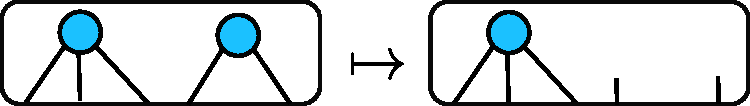
\includegraphics[scale=.4]{pictures/tensor-projection-1}}
\end{array}
$$
\end{itemize}
\end{minipage}
}
\caption{Prime functions for shallow terms.}\label{fig:prime-for-shallow-terms}
\end{figure}

\begin{figure}
\fbox{
\begin{minipage}{1\linewidth}
\begin{itemize}
\item \textbf{Unit.}
$$
\begin{array}{c}
 \ranked{\Sigma \ \ \to \ \ \reduce k \Sigma^k}\\[5pt]
        {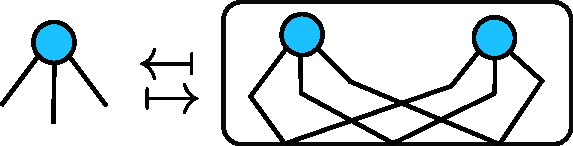
\includegraphics[scale=.4]{pictures/tensor-injection}}
\end{array}
$$
\item \textbf{Increase fold.}
$$
\begin{array}{c}
 \ranked{\reduce k \Sigma \ \ \to \ \ \reduce {k+1}\Sigma}\\[5pt]
        {
\includegraphics[scale=.4]{pictures/add-fold}}	
\end{array}$$
\item \textbf{Decrease fold.}
$$
\begin{array}{c}
 \ranked{\reduce {k+1} \Sigma \ \ \to \ \ \reduce {k}\Sigma+\bot}\\[5pt]
        {
\includegraphics[scale=.4]{pictures/reduce-fold}}	 
\end{array}$$
\item \textbf{projection of copairs.}
$$
\begin{array}{c}
   \ranked{\Sigma\product \Sigma \ \ \to \ \ \reduce 1 \Sigma}\\[5pt]
        {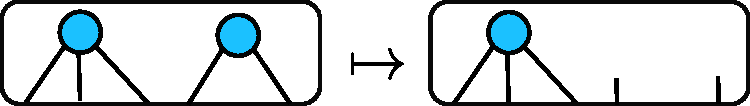
\includegraphics[scale=.4]{pictures/tensor-projection-1}}	
\end{array}$$
\end{itemize}
\end{minipage}
}
\caption{Additional prime functions for folds.}\label{fig:additional-prime-for-fold}
\end{figure}

\begin{figure}
\fbox{
\begin{minipage}{1\linewidth}
\begin{itemize}
\item \textbf{Folds over pairs.}
$$
\begin{array}{rll}
  \ranked{\reduce k (\Sigma_1 + \Sigma_2)}& \ranked{\to} & \ranked{\reduce k \Sigma_1 + \reduce k \Sigma_2}\\
         (a,i)/f & \mapsto & ((a/f),i)
\end{array}
$$
\item \textbf{Shallow terms over pairs.}
$$
\begin{array}{rll}
  {\shallowterm {(\Sigma_1 + \Sigma_2)} \Gamma} & \ranked{\to} & \ranked{(\shallowterm {\Sigma_1} \Gamma) + (\shallowterm {\Sigma_2} \Gamma)}\\
        (a,i)\tensorpair{t_1,\dots,t_n} &\mapsto& (a\tensorpair{t_1,\dots,t_n},i)
\end{array}
$$
\item \textbf{Shallow terms over copairs.}
$$
\begin{array}{c}
  \ranked{{\shallowterm {(\Sigma_1 \product \Sigma_2)} \Gamma}
   \ \  \to \ \ {(\shallowterm {\Sigma_1} \Gamma) \product (\shallowterm {\Sigma_2} \Gamma)}}\\[5pt]
        {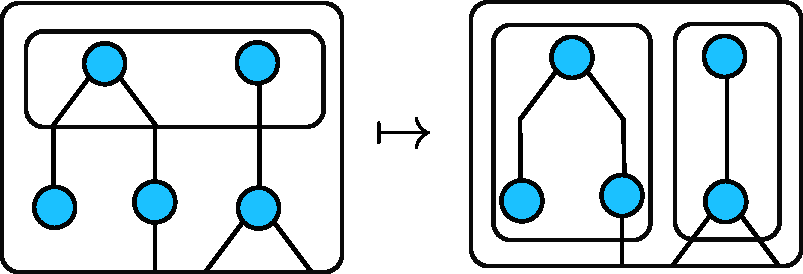
\includegraphics[scale=.4]{pictures/tensor-shallow-distrib}}
        \end{array}
$$
\item \textbf{Folds over copairs.}
$$
\begin{array}{c}
\ranked{(\reduce k \Sigma_1) \product (\reduce k {\Sigma_2}) \ \ \to \ \reduce k (\Sigma_1 \product \Sigma_2)}\\[5pt]
        {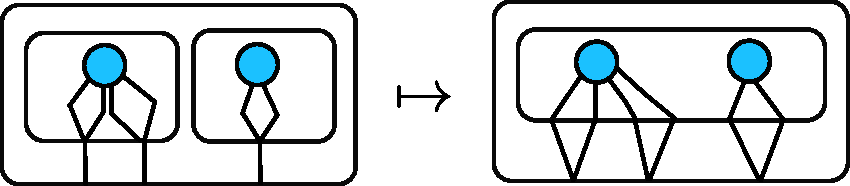
\includegraphics[scale=.4]{pictures/tensor-fold-distrib-2}}  
\end{array}
$$
\item \textbf{Folds over copairs (bis).}
$$
\begin{array}{c}
    \ranked{\reduce k (\Sigma_1 \product \Sigma_2) \ \ \to \ \ \reduce k ((\reduce k {\Sigma_1})\product (\reduce k \Sigma_2))}\\[5pt]
        {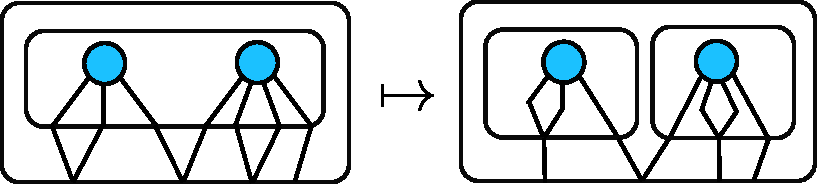
\includegraphics[scale=.4]{pictures/tensor-fold-distrib-1}}   
\end{array}
$$
\item \textbf{Shallow terms over folds.}
$$
\begin{array}{c}
 \ranked{\shallowterm \Sigma {\reduce k \Gamma}\ \ \to \ \ \reduce k (\shallowterm \Sigma {\Gamma})}\\[5pt]
 {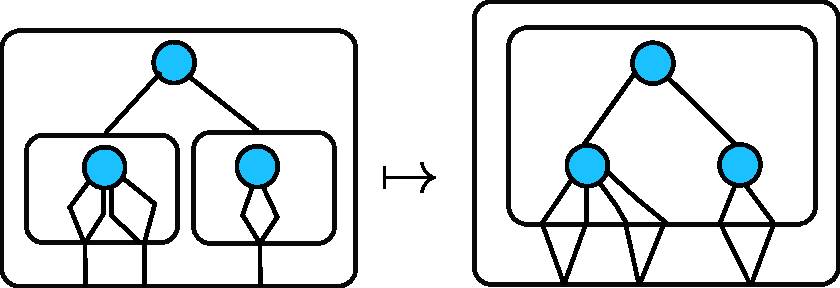
\includegraphics[scale=.4]{pictures/shallow-fold-distrib}} 
\end{array}
$$
\item \textbf{Folds over shallow terms.} 
$$
\begin{array}{c}
 \ranked{\reduce k \Sigma\cdot \Gamma\ \ \to \ \ (\reduce k \Sigma) \cdot \mati k \Gamma}\\[5pt]
 {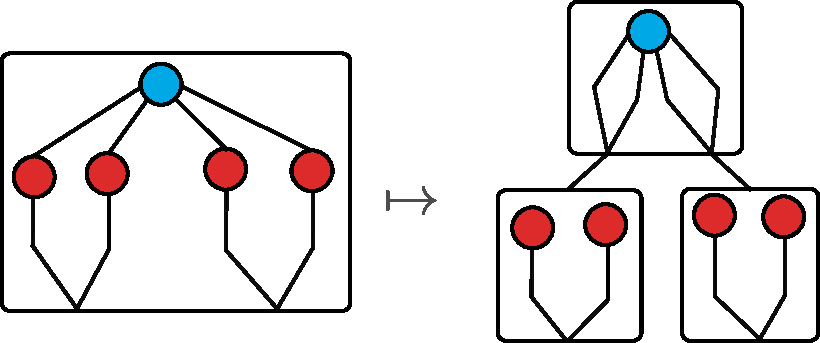
\includegraphics[scale=.4]{pictures/last-prime-function}} 
\end{array}
$$
$\rGamma$ is a set of unary elements.
\end{itemize}
\end{minipage}
}
\caption{Additional distributivity prime functions.} \label{fig:additional-distrib-prime}
\end{figure}

\begin{figure}
\fbox{
\begin{minipage}{1\linewidth}
\begin{itemize}
\item \textbf{Untwist.}
$$
\begin{array}{c}
\ranked{\tmonad {\reduce 1\Sigma} \ \  \to \ \ \reduce 1 \tmonad \Sigma}\\[5pt]
         {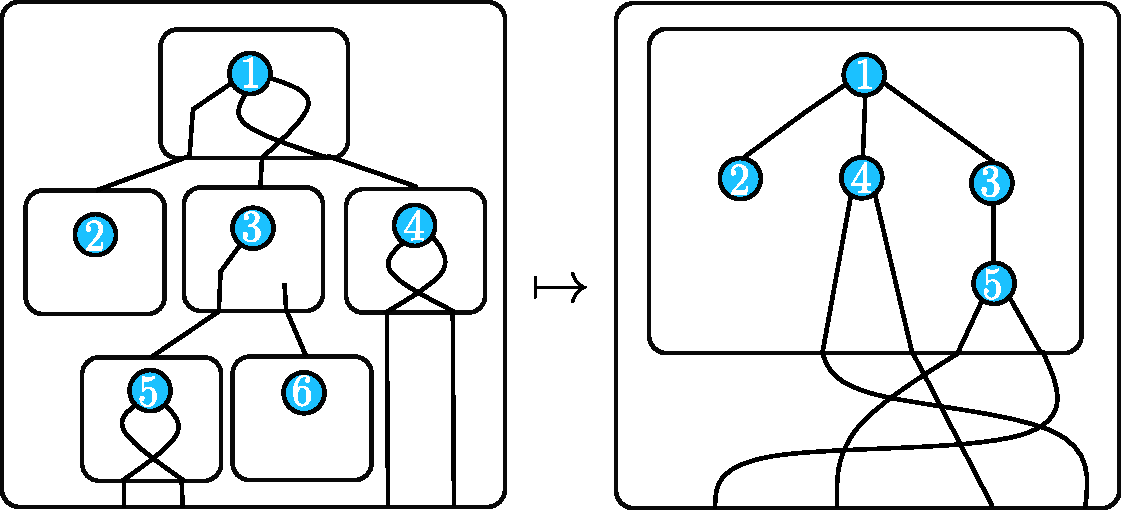
\includegraphics[scale=.4]{pictures/unfold-1}}
\end{array}
$$
\item \textbf{External fold.}
$$
\begin{array}{c}
\ranked{\tmonad {\reduce k\Sigma} \ \  \to \ \ \reduce k \tmonad \reduce k\Sigma}\\[5pt]
         {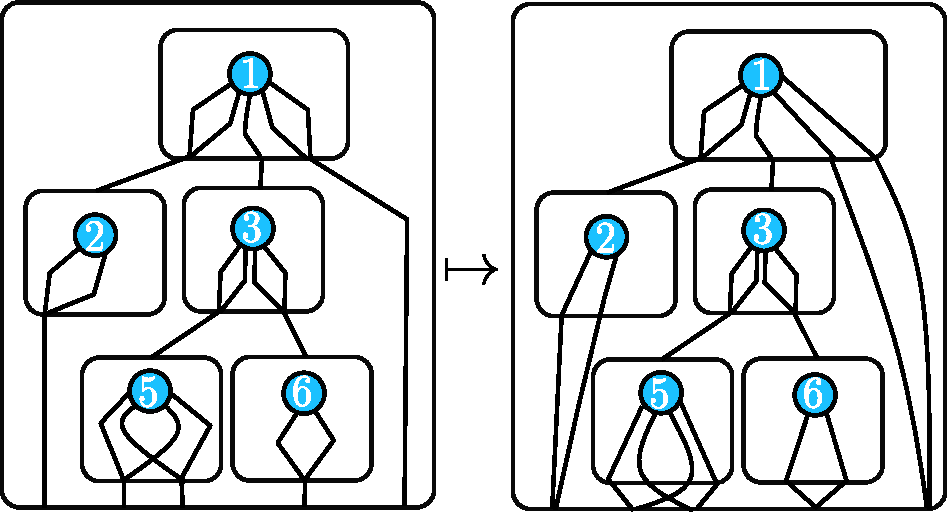
\includegraphics[scale=.43]{pictures/external-unfold-1}}
\end{array}
$$
\item \textbf{Matching.}
$$
\begin{array}{c}
\ranked{\shallowterm {\reduce k \Sigma}{\Gamma^k} \ \ \to \ \ \reduce 1(\shallowterm \Sigma \Gamma)}\\[5pt]
\includegraphics[scale=.3]{pictures/shallow-unfold}
\end{array}
$$
\end{itemize}
\end{minipage}
}
\caption{Weak forms of unfolding.}\label{fig:weak-unfolding}
\end{figure}

\subsection{The atomic functions not explained in Figure~\ref{fig:fo-term}}
\label{sec:atomic-and-combinators}
In this section, we define the atomic functions whose definitions were not given in Figure~\ref{fig:fo-term}. 

\subsubsection{Factorisations}
    Let $t \in \tmonad \rSigma$ be a term. 
    There are two equivalent definitions of factorisations of $t$. One definition is that a factorisation is an equivalence relation on non-port nodes where every equivalence class is a factor; the other definition is that it is any term $s  \in \tmonad \tmonad \rSigma$ which flattens to $t$. 
    The two definitions are easily seen to be equivalent, in the sense that there is a one-to-one correspondence between factorisation equivalences and factorisation terms.
    %  which is explained in the following picture:
    % \mypic{14}
    Suppose that $\ranked{\Sigma_1}$ and $\ranked{\Sigma_2}$ are ranked sets. The ancestor and descendant factorisations 
        \begin{align*}
            \overbrace{\ancfact}^{\text{ancestor}}, \overbrace{\decfact}^{\text{descendant}}  : \ranked{\tmonad(\Sigma_1+\Sigma_2) \to \tmonad(\tmonad \Sigma_1 + \tmonad \Sigma_2)}
        \end{align*}
        are defined as follows. Consider an input term
        \begin{align*}
            t \in \ranked{\tmonad(\Sigma_1+\Sigma_2)}.
        \end{align*}
        We say that two non-port nodes have \emph{same type} if both have labels in the same  $\ranked{\Sigma_i}$; otherwise we say that non-port nodes have \emph{opposing type}.  Call two non-port nodes \emph{ancestor equivalent}  if they have the same proper ancestors of opposing type. Call two non-port nodes \emph{descendant equivalent}  if they  are ancestor equivalent and they have the same proper descendants of opposing type. Here is a picture, with $\ranked{\Sigma_1}$ being red and $\ranked{\Sigma_2}$ being blue: 
        \begin{center}
      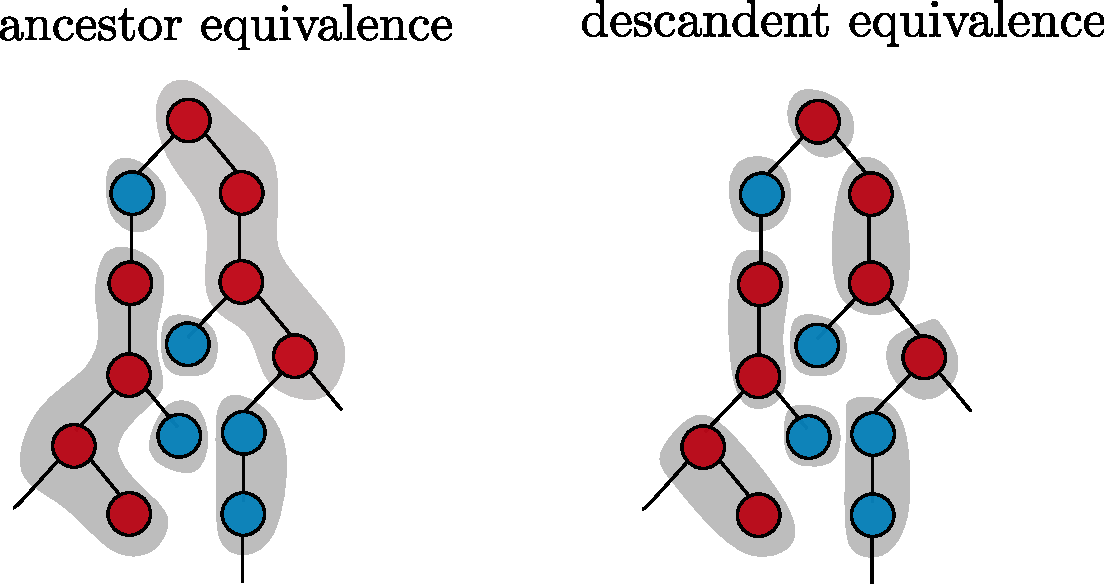
\includegraphics[scale=.4]{facto-up-down.pdf}
        \end{center}
        Both ancestor and descendant equivalences are factorisations; and in each case equivalence classes contain only nodes of same type.  The function $\ancfact$ maps a term to (the term of terms corresponding to) its ancestor equivalence relation, likewise we define $\decfact$ for  descendant factorisations.
    
        \subsubsection{Pre-order traversal.} The preorder traversal function  
        \begin{align*}
            \ranked{\preorder : \tmonad \Sigma \to \reduce 1 \tmonad (\rSigma + 0 + 2)}
        \end{align*}
        is the natural extension -- from trees to terms -- of the depth-first traversal, as explained below (the nullary grey nodes represent the labels from $\ranked 0$, and the binary grey nodes represent the labels from $\ranked 2$):
        \begin{center}
        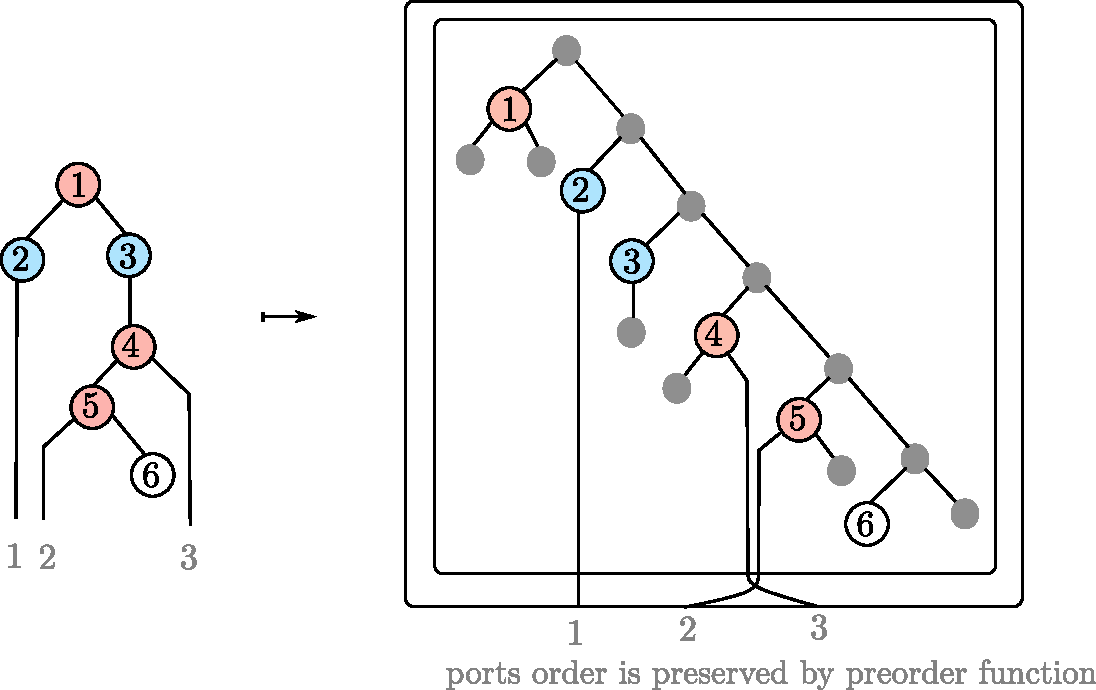
\includegraphics[scale=.45]{preorder.pdf}
        \end{center}
The $\preorder$ function respects the input port order, this is the reason  why we have a fold $\reduce 1$ in the output type. 
\subsubsection{Unfolding}
The general idea behind the  unfolding operation 
\begin{align*}
\ranked{
    \unfoldsmall : \shallowterm {(\reduce k   \Sigma)} {\Gamma^k} \to \reduce 1 (\shallowterm \Sigma \Gamma)
}
\end{align*} 
is to eliminate a $k$-fold by matching it with a $k$-th power. 
The unfolding operation is explained in the following picture for $k=2$: 
        \begin{center}
        \includegraphics[scale=.35]{shallow-unfold.pdf}
        \end{center}
% One of the main results in this paper will be  that an iterated version of the unfold operation, of type
% \begin{align*}
% \ranked{    \tmonad (\reduce k \Sigma^k) \to \reduce k (\tmonad \Sigma)^k,}
% \end{align*}
% can be derived from the other operations. 

% The formal definition is 
% \begin{align*}
% (a/f) \tensorpair{\tensorpair{b_{1,1},\ldots,b_{1,k}},\ldots,\tensorpair{b_{n,1},\ldots,b_{n,k}}} \qquad \mapsto \qquad 
% (a\tensorpair{b_{f(1)},\ldots,b_{f(\arity a)}})/g
% \end{align*}
% where $g$ is defined so that it matches ...

\noindent\begin{example}[Filter]\label{ex:filter} 
 To get a feeling for the atomic functions and combinators, we derive the function
$$ \ranked{f:\tmonad (\rSigma+\rGamma)\to\tmonad \rSigma}$$
discussed earlier, which erases the elements of $\rGamma$ from the input term, where $\rGamma$ is a finite set of unary symbols. 

Consider the atomic function $\ranked{\unit_\rSigma:\rSigma\to\tmonad\rSigma}$ and the constant function $\ranked{\mathrm{empty}:\rGamma\to\tmonad\rSigma}$ which associates to every element of $\rGamma$ the empty term. The function $\ranked{\mathrm{empty}}$ is atomic because its domain is finite. We start by lifting $\ranked{\unit_\rSigma}$ and $\ranked{\mathrm{empty}}$ to the type constructor $+$, then we compose the result with the atomic projection function as follows
\begin{align*}
\xymatrix{
    \ranked{\rSigma+\rGamma}\quad \ar[r]^-{\ranked{\unit_\Sigma+\mathsf{empty}}} & \quad \ranked{\tmonad\rSigma+\tmonad\rSigma}\ar[r]^-{} &\tmonad\rSigma
},
\end{align*}
We lift the obtained function to terms, and compose the result with the $\flatt_\rSigma$ function to obtain our function $\ranked{f}$.  
\end{example}

More examples of derived functions are given in Appendix.~\ref{sec:AppendixExamples}.